\documentclass[12pt]{article}
\usepackage[margin=1in]{geometry}
\usepackage[utf8]{inputenc}
\usepackage[spanish]{babel}
\usepackage{parskip}
\usepackage{setspace}
\usepackage{amsmath}
\usepackage{tikz}
\usepackage{graphicx}
\usepackage{hyperref} % Siempre debe ir al final.

% Opciones de Paquetes.
\decimalpoint % {babel}
\onehalfspacing % {setspace}
\usetikzlibrary{babel} % Para que tikz no conflictue con {babel} con figuras como "->".
\graphicspath{{./img/}} % {graphicx}

% Encabezado.
\title{Clase 33. Coordenadas Polares.}
\author{MIT 18.01: Single Variable Calculus.}
\date{}


\begin{document}

\maketitle

\begin{abstract}
\noindent En la Clase 27 revisamos brevemente el \textbf{sistema de coordenadas polares} y en ésta profundizaremos más sobre él. Estudiaremos la diferencia con el cartesiano, calcularemos áreas de figuras y veremos algunas gráficas obtenidas bajo este sistema.
\end{abstract}


\section{Coordenadas Polares.}

Como recordaremos de la Clase 27, el sistema de coordenadas polares es aquel donde la ubicación de un punto $P$ es explicado por:

\begin{enumerate}
\item La \textbf{distancia} $r$ de $P$ hacia el origen $O$ (también conocido como polo).
\item La \textbf{dirección} de $P$ dada por un ángulo $\theta$ medido entre un rayo y el segmento $\overline{OP}$.
\end{enumerate}

\begin{figure}[hbt!]
\centering

\begin{tikzpicture}
% Grids de ayuda.
%\draw [help lines] (-5, -1) grid (5, 3);

% Coordenada Polar
\draw [->, line width = 0.3mm] (-2, 0) -- (2, 0) node [right] {$x$ (rayo)};
\draw [fill = black, line width = 0.3mm]
  (-2, 0) node [left, align = center] {(polo)\\$O$} -- node [above] {$r$} (1.5, 2.5) circle (0.8mm) node [right]{$P(r, \ \theta)$};
\draw [->, line width = 0.25mm] (0.1, 0) arc (0:50:1.45cm);
\node at (0.3, 0.65) {$\theta$};
\end{tikzpicture}

\caption{Coordenada polar $P(r, \ \theta)$.}
\end{figure}

Como iremos viendo, las coordenadas polares involucran la geometría del círculo puesto que la dirección del punto irá dándose a partir de un ángulo $\theta$ medido en radianes.

\subsection{Relación entre coordenadas polares y cartesianas.}

Es posible relacionar los sistemas de coordenadas polar y cartesiano (también conocido como rectangular), lo cual geométricamente se puede lograr al unirlos en sus orígenes.

\newpage

\begin{figure}[hbt!]
\centering

\begin{tikzpicture}
%\draw [help lines] (-6, -6) grid (6, 6);

\draw [<->, line width = 0.3mm] (-3.5, 0) -- (3.5, 0) node [below] {$x$} node [above] {$\theta = 0$};
\draw [<->, line width = 0.3mm] (0, -3.5) -- (0, 3.5) node [left] {$y$} node [right] {$\theta = \pi/2$};
\draw (0, 0) circle (3cm);

\draw [line width = 0.3mm, fill = black] (0, 0) -- node [above] {$r$} (2.12, 2.12) circle (0.65mm) node [right] {$P(x, \ y) = P(r, \ \theta)$};
\draw [dashed] (0, 0) -- node [below] {$x$} (2.12, 0) -- node [right] {$y$} (2.12, 2.12);
\draw [->, line width = 0.25mm] (1.2, 0) arc (0:35:1.5cm);
\draw (2.12, 0.3) -- (1.82, 0.3) -- (1.82, 0);

\node at (-0.2, -0.25) {$0$}; % Origen.
\node at (0.7, 0.32) {$\theta$};

\end{tikzpicture}

\caption{Relación entre los sistemas de coordenadas polar y rectangular.}

\end{figure}

A partir de esta relación entre los sistemas de coordenadas polar y rectangular, es posible obtener las siguientes cuatro ecuaciones:
\begin{align*}
  &(1) \ x = r \cos(\theta)       & &(2) \ y = r \sin(\theta) \\
  &(3) \ r = \pm \sqrt{x^{2} + y^{2}} & &(4) \ \theta = \tan^{-1}\left(\frac{y}{x}\right) = \tan^{-1}\left(\frac{-y}{-x}\right)
\end{align*}
Por medio de estas ecuaciones podemos convertir un punto desde un sistema de coordenadas a otro, como es resumido en la siguiente tabla:

\begin{table}[hbt!]
\centering

\begin{tabular}{c c}
\hline
\hline
Ecuaciones & Conversión de coordenadas \\
\hline
$(1)$ y $(2)$ & Polar $\rightarrow$ Rectangular \\
$(3)$ y $(4)$ & Rectangular $\rightarrow$ Polar \\
\hline
\hline
\end{tabular}

\end{table}

Observemos que al pasar un punto \textbf{desde un sistema de coordenadas polar a uno rectangular} (ecuaciones $(1)$ y $(2)$), la coordenada $y$ no está en función de $x$. Ambas son paramétricas en términos de $\theta$, por tanto cada punto $(x, \ y)$ resultante solo describe su posición en $x$ y en $y$ unidades con respecto al origen\footnote{Es decir, actúan más como una etiqueta del plano cartesiano/rectangular.}.

Por otra parte, al convertir un punto \textbf{desde un sistema rectangular a uno polar} (ecuaciones $(3)$ y $(4)$), es posible que $r$ sea negativa y $\theta$ puede ser expresado de varias formas ya que crece en el intervalo $[0, \ 2\pi]$. Esto depende del cuadrante en el que está $(x, \ y)$, por lo que es aconsejable revisar si la posición de $(r, \ \theta)$ es consistente con el del punto anterior\footnote{Esto no es necesario con las ecuaciones $(1)$ y $(2)$. Sus resultados siempre serán únicos.}.

\subsection{Planos cartesiano y polar.}

Acabamos de explicar la interpretación de las coordenadas cartesiana y polar en la subsección anterior, pero ahora veámoslo de manera más geométrica a partir de sus planos.

\begin{figure}[hbt!]

\centering

\begin{tikzpicture}
%\draw [color = gray!30] (-8, -3) grid (8, 3);

% Plano Cartesiano.
\draw [<->, line width = 0.3mm] (-8, 0) -- (-2, 0) node [right] {$x$};
\draw [<->, line width = 0.3mm] (-5, -3) -- (-5, 3) node [right] {$y$};
\node at (-5.2, -0.25) {$0$};

\draw [color = gray] (-8, 1) -- (-2, 1) node [right, color = black] {$y = 1$};
\draw [color = gray] (-8, -1.5) -- (-2, -1.5) node [right, color = black] {$y = -1.5$};

\draw [color = gray] (-3, -3) node [below, color = black] {$x = 2$} (-3, -3) -- (-3, 3);
\draw [color = gray] (-6, -3) node [below, color = black] {$x = -1$} (-6, -3) -- (-6, 3);

% Plano polar.
\draw (4.5, 0) circle (1cm);
\draw (4.5, 0) circle (2.5cm);
\node at (4.5, -0.35) {$O$};

\draw [->, line width = 0.25mm] (4.5, 0) -- (7.5, 0) node [above] {$\theta = 0$};
\draw [->, line width = 0.25mm] (4.5, 0) -- (4.5, 3) node [right] {$\theta = \pi/2$};
\draw [->, line width = 0.25mm] (4.5, 0) -- (2.5, -2);
\draw [->, line width = 0.25mm] (4.5, 0) -- (6.5, -2) node [below] {$\theta = -\pi/4$};

\node at (3, 0.2) {$r = 1$};
\node at (1.8, 1.5) {$r = 2.5$};
\end{tikzpicture}

\caption{Planos de coordenadas cartesiano (izq) y polar (der).}

\end{figure}

Como vemos en la imagen de arriba, un punto en el plano cartesiano nos indica su distancia del origen con respecto a $x$ e $y$. De modo similar, un punto en el sistema polar también nos entrega información sobre qué tan alejado está del polo $O$ ($r$), pero se añade la dirección en que se mueve ($\theta$). Si $\theta$ es negativo, lo está haciendo en dirección de las agujas del reloj.

\textbf{Ejemplo 1.} Convierta el punto $(x, \ y) = (1, \ -1)$ a coordenada polar $(r, \ \theta)$ y encuentre los valores posibles que puede tomar.

\textbf{Solución.} Debido a la ambigüedad en el resultado a obtener al convertir una coordenada rectangular a uno polar, primero grafiquemos el punto $(1, \ -1)$ para conocer su cuadrante.

\begin{figure}[hbt!]

\centering

\begin{tikzpicture}
%\draw [color = gray!50] (-4, -2.5) grid (4, 2.5);

\draw [<->, line width = 0.25mm] (-2.5, 0) -- (2.5, 0) node [below] {$x$};
\draw [<->, line width = 0.25mm] (0, -2.5) -- (0, 2.5) node [left] {$y$};

\draw [dashed, color = gray] (0, -1) node [left, color = black] {$-1$} -- (1, -1) -- (1, 0) node [above, color = black] {$1$};
\draw [fill = black] (1, -1) circle (0.6mm) node [right] {$(1, \ -1)$};
\end{tikzpicture}

\end{figure}

Como se puede apreciar en el gráfico de arriba, el punto $(1, \ -1)$ está en el cuarto cuadrante.

Luego, procedamos a calcular a $r$.
\[
  r = \pm \sqrt{x^{2} + y^{2}} = \pm \sqrt{1^{2} + (-1)^{2}} = \pm \sqrt{2}
\]
Posteriormente, obtengamos el valor del $\angle \theta$.
\[
  \theta = \tan^{-1}\left(\frac{-1}{1}\right) = \tan^{-1}(-1) = - \frac{\pi}{4}
\]
El valor de $\theta$ nos muestra que el punto se mueve en un ángulo de $\pi/4$ en favor de las agujas del reloj. Por lo tanto, para ser consistente con el punto en el plano cartesiano, su distancia con el polo debe ser $r = \sqrt{2}$.

\begin{figure}[hbt!]
\centering

\begin{tikzpicture}
%\draw [color = gray!50] (-4, -3) grid (4, 3);

\draw [->, line width = 0.25mm] (0, 0) node [left] {$O$} -- (3, 0) node [right] {$\theta = 0$};

\draw [line width = 0.25mm, fill = black] (0, 0) -- (1.4, -1.3) circle (0.6mm) node [right] {$(\sqrt{2}, \ -\pi/4)$};
\draw [->, line width = 0.25mm] (1, 0) arc (0:-35:1.2);
\node at (2, -0.5) {$\theta = - \pi/4$};
\end{tikzpicture}

\end{figure}

Si mantenemos a $r = \sqrt{2}$, podemos ver que es posible llegar a la misma posición donde está el punto en la imagen de arriba, pero moviéndonos en dirección contra reloj. Es decir, se debe cumplir que:
\begin{align*}
\frac{\pi}{4} + \theta &= 2\pi \\
\theta &= \frac{7\pi}{4}
\end{align*}
Recordemos que $\theta$ lo obtenemos a partir de la función inversa que nos da la relación entre $y$ y $x$, la cual es $\tan^{-1}(\cdot)$. En este ejemplo, dicha relación es $-1$, por lo que para saber si el $\angle \theta = 7\pi/4$ es el correcto, también debe cumplirse ese valor al calcular la $\tan(\theta)$.
\[
  \tan\left(\frac{7\pi}{4}\right) = -1
\]
Como vemos, la relación entre $y$ y $x$ sigue siendo igual a $-1$ para $\theta = 7\pi/4$, lo cual también podemos ver de forma gráfica.

\begin{figure}[hbt!]
\centering

\begin{tikzpicture}
%\draw [color = gray!50] (-4, -3) grid (4, 3);

\draw [->, line width = 0.25mm] (0, 0) node [left] {$O$} -- (3, 0) node [right] {$\theta = 0$};

\draw [line width = 0.25mm, fill = black] (0, 0) -- (1.4, -1.3) circle (0.6mm) node [right] {$(\sqrt{2}, \ 7\pi/4)$};
\draw [->, line width = 0.25mm] (1, 0) arc (0:324:1.2); % Ángulo final: (360-35) - 1
\node at (-0.7, -1.5) {$\theta = 7\pi/4$};
\end{tikzpicture}

\end{figure}

Ahora, también es posible que $r = - \sqrt{2}$. Que $r < 0$ quiere decir que su distancia desde el polo a $(r, \ \theta)$ es $r = \sqrt{2}$, pero en \textbf{sentido contrario}. Por lo tanto, nuestra tarea es buscar un $\angle \theta$ para calcular a $r$ de forma paralela y opuesta a la coordenada polar.

Geométricamente, lo que podemos hacer es buscar un $\angle \theta$ tal que su suma con $\pi/4$ sea $\pi$, ya que buscamos que la dirección de la distancia sea paralela con el punto $(r, \ \theta)$.

\begin{figure}[hbt!]

\centering

\begin{tikzpicture}
%\draw [color = gray!50] (-4, -3) grid (4, 3);

\draw [->, line width = 0.25mm] (0, 0) node [left] {$O$} -- (3, 0) node [right] {$\theta = 0$};

\draw [line width = 0.25mm, dashed, fill = black] (0, 0) -- (1.4, -1.3) circle (0.6mm) node [right] {$(-\sqrt{2}, \ \theta)$};
\draw [line width = 0.25mm, fill = black] (0, 0) -- (-1.4, 1.3);

\draw [->, line width = 0.25mm] (1, 0) arc (0:-35:1.2);
\draw [->, line width = 0.25mm] (1, 0) arc (0:130:1.2); % Ángulo final: (180-35) - 15

\node at (2, -0.5) {$\theta = - \pi/4$};
\node at (0, 0.5) {$\theta$};
\end{tikzpicture}

\end{figure}

Por lo tanto:
\begin{align*}
  \frac{\pi}{4} + \theta &= \pi \\
  \theta &= \frac{3\pi}{4}
\end{align*}
Podemos ver que es $\theta = 3\pi/4$ es el ángulo correcto al verificar que su tangente es igual a $-1$.
\[
  \tan\left(\frac{3\pi}{4}\right) = -1
\]
A continuación tenemos la gráfica anterior actualizada.

\begin{figure}[hbt!]

\centering

\begin{tikzpicture}
%\draw [color = gray!50] (-4, -3) grid (4, 3);

\draw [->, line width = 0.25mm] (0, 0) node [left] {$O$} -- (3, 0) node [right] {$\theta = 0$};
\draw [line width = 0.25mm, dashed, fill = black] (0, 0) -- (1.4, -1.3) circle (0.6mm) node [right] {$(-\sqrt{2}, \ 3\pi/4)$};
\draw [line width = 0.25mm, fill = black] (0, 0) -- (-1.4, 1.3);
\draw [->, line width = 0.25mm] (1, 0) arc (0:130:1.2); % Ángulo final: (180-35) - 15
\node at (1, 1.4) {$\theta = 3\pi/4$};
\end{tikzpicture}

\end{figure}

Así, al convertir a coordenada polar al punto $(x, \ y) = (1, \ -1)$, es posible expresarlo de las siguientes tres maneras, los cuales son todos consistentes con el original:
\[
  P(r, \ \theta) = \left\{
                     \left(\sqrt{2}, \ -\frac{\pi}{4}\right); \quad
                     \left(\sqrt{2}, \ \frac{7\pi}{4}\right); \quad
                     \left(-\sqrt{2}, \ \frac{3\pi}{4}\right)
                   \right\}
\]
Para evaluar que lo sean, podemos usar las ecuaciones $(1)$ y $(2)$ vistas en la subsección anterior para convertirlas a coordenadas rectangulares. Por ejemplo:
\begin{align*}
  x &= \sqrt{2} \cdot \cos\left(-\frac{\pi}{4}\right) = 1 \\
  y &= \sqrt{2} \cdot \sin\left(-\frac{\pi}{4}\right) = -1
\end{align*}

\subsection{Ecuaciones Polares.}

Así como podemos obtener puntos, también podemos formar curvas con un conjunto de ellos en el sistema de coordenadas polares. La expresión algebraica que nos permite aquello, se conoce como \textbf{Ecuación Polar} y suele representarse\footnote{Aunque su forma general es $F(r, \ \theta) = 0$.} como $r = f(\theta)$.

En otras palabras, la gráfica de una ecuación polar consiste de todos los puntos $(r, \ \theta)$ que satisfacen la igualdad $r = f(\theta)$.

Las ecuaciones polares más básicas, son aquellas donde $r$ o $\theta$ son constantes. La igualdad $r = a$, cuando la constante $a > 0$, corresponde a un círculo de radio $a$ con su centro en el origen. Es decir, obtenemos dicha figura si mantenemos fijo a $r$ y $\theta$ varía en $[0, \ 2\pi)$.

Lo anterior también podemos demostrarlo usando su fórmula para convertir coordenadas rectangulares a polares.
\[
  a = \sqrt{x^{2} + y^{2}}
\]

\begin{figure}[hbt!]
\centering

\begin{tikzpicture}
%\draw [color = gray!30] (-8, -3) grid (8, 3);

% Plano Polar.
\draw [color = gray!70] (-4, 0) circle (2.5cm);
\draw [color = gray!70] (-6, -2) -- (-2, 2) node [right, color = black] {$\theta = \pi/4$};
\draw [color = gray!70] (-4, -2.8) -- (-4, 2.8) node [above, color = black] {$\theta = \pi/2$};
\draw [color = gray!70] (-2, -2) -- (-6, 2);
\draw [color = gray!70] (-4, 0) -- (-7, 0) node [left, color = black] {$\theta = \pi$};

\draw [line width = 0.25mm] (-4, 0) circle (1.5cm);
\draw [->, line width = 0.25mm] (-4, 0) -- (-1, 0) node [right] {$\theta = 0$};

\node at (-3.3, 1.65) {$r = a$};

%Plano cartesiano.
\draw [color = gray!60] (1.5, -2.5) grid (6.5, 2.5);
\draw [<->, line width = 0.25mm] (1.5, 0) -- (6.5, 0) node [right] {$x$};
\draw [<->, line width = 0.25mm] (4, -2.5) -- (4, 2.5) node [right] {$y$};

\draw [line width = 0.25mm] (4, 0) circle (1.5cm);

\node at (5.65, -0.2) {$a$};
\node at (3.8, -0.25) {$0$};
\node at (5.6, 1.7) {$x^{2} + y^{2} = a^{2}$};

\end{tikzpicture}

\caption{Representación polar (izq) y cartesiana (der) de la ecuación polar $r = a$.}

\end{figure}

En cuanto a la ecuación polar $\theta = c$, con $c =$ constante, los puntos $(r, \ \theta)$ forman una recta que pasa por el origen y con una inclinación dada por dicho ángulo. Es decir, $\theta$ está fijo y $r$ varía en $(-\infty, \ \infty)$. Si $\theta = c$ forma un rayo, entonces $r$ toma valores en $[0, \ \infty)$.

La representación de la ecuación polar $\theta = c$ en coordenadas rectangulares se obtiene a partir de su tangente, ya que describe la relación de dicho ángulo con $y$ y $x$. Por lo tanto,
\begin{align*}
  \tan(c) &= \frac{y}{x} \\
  y &= \tan(c)x
\end{align*}
Como $\tan(c) =$ constante, entonces $y = \tan(c)x$ es una función lineal cuya inclinación está dada por $\theta = c$.

\begin{figure}[hbt!]
\centering

\begin{tikzpicture}
%\draw [color = gray!30] (-8, -3) grid (8, 3);

% Plano Polar.
\draw [line width = 0.25mm] (-6, 0) node [below] {$O$} -- (-2.9, 2.3) node [right] {$\theta = c$};

\draw [->, line width = 0.25mm] (-6, 0) -- (-3, 0) node [right] {$\theta = 0$};
\draw [->, line width = 0.25mm] (-4.3, 0) arc (0:35:1.7cm);

\node at (-3.8, 0.55) {$\theta = c$};
\node [rotate = 38] at (-4.5, 1.5) {$0 \leq r < \infty$};

%Plano cartesiano.
\draw [color = gray!60] (0.8, -1.2) grid (6.5, 2.5);
\draw [<->, line width = 0.25mm] (1, 0) -- (5.5, 0) node [right] {$x$};
\draw [<->, line width = 0.25mm] (3, -1) -- (3, 2.5) node [right] {$y$};

%\draw [line width = 0.25mm] (4, 0) circle (1.5cm);
\draw [line width = 0.25mm] (3, 0) -- (6.1, 2.3) node [above] {$y = \tan(c)x$};
\draw [->, line width = 0.25mm] (4.7, 0) arc (0:35:1.7cm);

\node [rotate = 38] at (4.5, 1.5) {$0 \leq x < \infty$};
\node at (5.3, 0.55) {$\theta = c$};
\node at (2.8, -0.25) {$0$};

\end{tikzpicture}

\caption{Representación polar (izq) y cartesiana (der) de la ecuación polar del rayo $\theta = c$.}

\end{figure}

En general, al trabajar con ecuaciones y coordenadas polares, se suelen usar los siguientes intervalos para $r$ y $\theta$:

\begin{table}[hbt!]
\centering

\begin{tabular}{c|c}
Variable & Intervalo(s) \\
\hline
$r$ & $[0, \ \infty)$ \\
$\theta$ & $(-\pi, \ \pi]$ o $[0, \ 2\pi)$
\end{tabular}

\end{table}

Las ecuaciones polares también podemos convertirlas a ecuaciones rectangulares/cartesianas y viceversa, con las mismas fórmulas que vimos para realizar dichas transformaciones con puntos.

\textbf{Ejemplo 2.} Sea $y = 1$ una ecuación cartesiana. Conviértala a una polar.

\textbf{Solución.} Podemos comenzar con el hecho de que $y = r \sin(\theta)$. Por lo tanto:
\[
  r \sin(\theta) = 1
\]
Como una ecuación polar es de la forma $r = f(\theta)$, entonces despejamos a $r$ en la igualdad de arriba.
\[
  r = \frac{1}{\sin(\theta)} = \csc(\theta)
\]
La solución que acabamos de obtener significa que, para cada valor de $\theta$ donde $\sin(\theta) \neq 0$, encontraremos un punto cuya distancia del polo es $r(\theta)$. Lo interesante es que si graficamos todas esas coordenadas $(r(\theta), \theta)$, veremos que la figura que se forma es la recta $y = 1$.

\begin{figure}[hbt!]

\centering

\begin{tikzpicture}
%\draw [color = gray!50] (-6, -3) grid (6, 3);

\draw [<->, line width = 0.25mm] (-3.2, 0) -- (3.2, 0) node [below] {$x$};
\draw [->, line width = 0.25mm] (0, 0) node [below] {$0$} -- (0, 2.5) node [right] {$y$};

\draw [color = blue, line width = 0.2mm] (-3, 1.5) -- (3, 1.5) node [right] {$y = 1$};

\draw [dashed, fill = black] (0, 0) -- (2.6, 1.5) circle (0.6mm);
\draw [dashed, fill = black] (0, 0) -- (1.3, 1.5) circle (0.6mm);
\draw [dashed, fill = black] (0, 0) -- (-0.5, 1.5) circle (0.6mm);
\draw [dashed, fill = black] (0, 0) -- (-2, 1.5) circle (0.6mm);

\draw [->, line width = 0.25mm] (1.5, 0) arc (0:30:1.4cm);
\node at (1, 0.25) {$\theta$};

\end{tikzpicture}

\end{figure}

En ocasiones siempre tendremos que considerar el intervalo de valores de $\theta$ para los cuales está definida la función $r(\theta)$ (i.e, su dominio). En este caso, como dijimos antes, es en donde $\sin(\theta) \neq 0$ y esto ocurre en $0 < \theta < \pi$. Más adelante veremos que esto es relevante para poder calcular integrales definidas con ecuaciones polares.

\textbf{Ejemplo 3.} Encuentre la ecuación polar para el siguiente círculo con centro $C(a, \ 0)$ y el intervalo de $\theta$ para el cual está definida.

\begin{figure}[hbt!]
\centering

\begin{tikzpicture}
%\draw [color = gray!60] (-4, -2) grid (4, 4);

\draw [<->, line width = 0.25mm] (-1, 0) -- (4, 0) node [below] {$x$};
\draw [<->, line width = 0.25mm] (0, -2) -- (0, 2) node [right] {$y$};

\draw [line width = 0.25mm] (1.5, 0) circle (1.5cm);

\node at (1.5, -0.25) {$a$};
\node at (3.3, -0.25) {$2a$};
\node at (-0.2, -0.25) {$0$};
\end{tikzpicture}

\end{figure}

\textbf{Solución.} Primero tenemos que buscar la ecuación cartesiana de la figura de arriba, la cual corresponde\footnote{La ecuación de cualquier círculo con centro en $C(h, \ k)$ es $r^{2} = (x - h)^{2} + (y - k)^{2}$, donde $r$ es su radio.} a:
\[
  a^{2} = (x - a)^{2} + (y - 0)^{2}
\]
Luego, tenemos que convertir esta ecuación rectagular a una polar. Un camino sería hacer de inmediato el reemplazo $x = r \cos(\theta)$ e $y = r \sin(\theta)$, pero uno más rápido es antes calcular los binomios cuadráticos y simplificar la ecuación.
\begin{align*}
  a^{2} &= x^{2} - 2ax + a^{2} + y^{2} \\
  0 &= x^{2} + y^{2} - 2ax
\end{align*}
Ahora transformemos esta igualdad a una polar, haciendo el reemplazo en $r^{2} = x^{2} + y^{2}$ y en $x = r \cos(\theta)$.
\begin{align*}
  0 &= r^{2} - 2a(r \cos(\theta)) \\
  r^{2} &= 2a r \cos(\theta) \\
  r &= 2a \cos(\theta)
\end{align*}
Para ver con cuál intervalo de $\theta$ obtenemos al círculo de la ecuación $r = 2a \cos(\theta)$, démosle valores al ángulo y calculemos los de salida. Usemos $\theta = 0$ y $\theta = \pi/2$, puesto que sabemos que $\cos(0) = 1$ y $\cos(\pi/2) = 0$.

\begin{table}[hbt!]
\centering

\begin{tabular}{c|c c}
$\theta$ & $0$ & $\pi / 2$ \\
\hline
$r(\theta)$ & $2a$ & $0$
\end{tabular}

\end{table}

Es decir, moviéndonos a contra reloj, con el intervalo $0 \leq \theta \leq \pi / 2$ obtenemos la mitad superior del círculo. Por lo tanto, la otra parte podemos encontrarla yendo en dirección a favor de las agujas del reloj usando los mismos valores. En otras palabras, en el intervalo $-\pi/2 \leq \theta \leq 0$.

\begin{table}[hbt!]
\centering

\begin{tabular}{c|c c}
$\theta$ & $0$ & $-\pi / 2$ \\
\hline
$r(\theta)$ & $2a$ & $0$
\end{tabular}

\end{table}

En consecuencia, la ecuación polar $r(\theta) = 2a \cos(\theta)$ está definida para $-\pi/2 \leq \theta \leq \pi/2$.


\section{Áreas de Ecuaciones Polares.}

Al trabajar con una función (o ecuación) polar, podría ser de nuestro interés conocer el área bajo su curva para un intervalo determinado.

Digamos que queremos calcular el área bajo la curva de $r = f(\theta)$ entre $[\theta = a, \ \theta = b]$.

\newpage

\begin{figure}[hbt!]
\centering
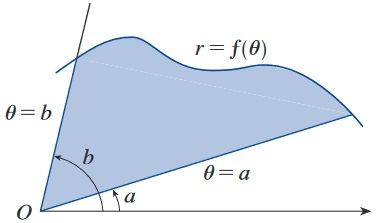
\includegraphics[scale=0.65]{01_area-ec-polar.jpg}
\caption{Stewart, J (2017). \textit{Cálculo. Trascendentes Tempranas}. Pp 669 (Modificada).}
\end{figure}

Para ello, primero dividimos el área bajo $r = f(\theta)$ en \textbf{sectores circulares} de ancho $\Delta \theta = \theta_{i} - \theta_{i - 1}$ y tomamos un ángulo $\theta_{i}^{*} \in [\theta_{i - 1}, \ \theta_{i}]$ tal que la distancia entre el polo y la curva es $f(\theta^{*})$.

\begin{figure}[hbt!]
\centering
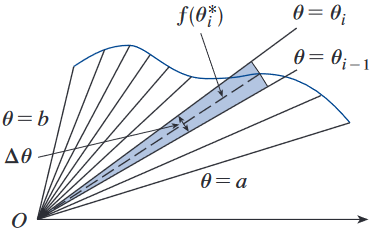
\includegraphics[scale=0.5]{02_area-ec-polar.jpg}
\caption{Stewart, J (2017). \textit{Cálculo. Trascendentes Tempranas}. Pp 669.}
\end{figure}

El sector circular es una porción de área $A$ de un círculo formado por dos radios y el arco que se forma entre ellos, calculado como el producto entre la proporción del $\angle \theta$ con respecto al del círculo y el área de la misma figura.

\begin{figure}[hbt!]

\centering

\begin{tikzpicture}
%\draw [color = gray!50] (-8, -3) grid (8, 3);

\draw [line width = 0.25mm] (-2, 0) circle (2cm);
\draw [line width = 0.25mm, fill = blue!40] (-0.28, -1) -- node [below] {$r$} (-2, 0) node [left] {$O$} -- node [above] {$r$} (-0.28, 1) arc (30:-30:2cm);

\node at (-1.4, 0) {$\theta$};

\draw [->] (-0.4, 0) -- (1.8, 0);
\node [draw] at (4.3, 0) {$\displaystyle A = \left(\frac{\theta}{2\pi}\right) \cdot (\pi r^{2}) = \frac{1}{2} r^{2} \theta$};
\end{tikzpicture}

\end{figure}

Por lo tanto, tomando la idea señalada arriba para la figura de $r = f(\theta)$, el $i$-ésimo sector circular $A_{i}$ lo calculamos como:
\[
  A_{i} \approx \frac{1}{2} [f(\theta^{*})]^{2} \Delta \theta
\]
Para obtener el área bajo la curva de $r = f(\theta)$ entre $[\theta = a, \ \theta = b]$, sumamos los $n$-ésimos sectores circulares $A_{i}$ y evaluamos su límite a medida que $n \to \infty$, con el fin de tener una mejor aproximación.
\[
  \lim_{n \to \infty} \sum_{i = 1}^{n} \frac{1}{2} [f(\theta^{*})]^{2} \Delta \theta = \int_{a}^{b} \frac{1}{2} [f(\theta)]^{2} d\theta
\]
En otras palabras, el área bajo la curva $A$ de una ecuación polar se obtiene a partir de la fórmula:
\[
  \int_{\theta = a}^{\theta = b} \frac{1}{2} [f(\theta)]^{2} d\theta
\]

\textbf{Ejemplo 4.} En el Ejemplo 3 encontramos que la figura que vemos a continuación resulta de la función polar $r = 2a \cos(\theta)$. Ahora calculemos el área bajo su curva.

\begin{figure}[hbt!]
\centering

\begin{tikzpicture}
%\draw [color = gray!60] (-4, -2) grid (4, 4);

\draw [<->, line width = 0.25mm] (-1, 0) -- (4, 0) node [below] {$x$};
\draw [<->, line width = 0.25mm] (0, -2) -- (0, 2) node [right] {$y$};

\draw [line width = 0.25mm] (1.5, 0) circle (1.5cm);

\node at (1.5, -0.25) {$a$};
\node at (3.3, -0.25) {$2a$};
\node at (-0.2, -0.25) {$0$};
\end{tikzpicture}

\end{figure}

\textbf{Solución.} En el ejemplo anterior también la ecuación $r = 2a \cos(\theta)$ está definida en el intervalo $-(\pi/2) < \theta < \pi/2$. Por lo tanto, el área bajo la curva de $r(\theta)$ lo calculamos como:
\[
  \int_{-\pi/2}^{\pi/2} \frac{1}{2} \left(2a \cos(\theta)\right)^{2} d\theta = \int_{-\pi/2}^{\pi/2} \frac{1}{2} 4a^{2} \cos^{2}(\theta) d\theta
                                                                             = 2a^{2} \cdot \int_{-\pi/2}^{\pi/2} \cos^{2}(\theta) d\theta
\]
Realicemos una sustitución trigonométrica, primero a partir de la identidad $\cos^{2}(\theta) = (1/2) (1 + \cos(2\theta))$
\[
  2a^{2} \cdot \int_{-\pi/2}^{\pi/2} \cos^{2}(\theta) d\theta = 2a^{2} \cdot \int_{-\pi/2}^{\pi/2} \frac{1}{2} (1 + \cos(2\theta)) d\theta
                                                              = a^{2} \cdot \int_{-\pi/2}^{\pi/2} (1 + \cos(2\theta)) d\theta
\]
y luego, estableciendo que $u = 2\theta$, implicando que $du = 2 d\theta$. Esto nos permite reescribir la integral de arriba como:
\[
  a^{2} \cdot \int_{-\pi/2}^{\pi/2} (1 + \cos(2\theta)) d\theta = a^{2} \cdot \int_{u = -\pi}^{u = \pi} \frac{1}{2} (1 + \cos(u)) du
                                                                = \frac{a^{2}}{2} \cdot \int_{-\pi}^{\pi} (1 + \cos(u)) du
\]
Al resolver la antiderivada y haciendo el reemplazo para retomar la variable original $\theta$, obtenemos lo siguiente:

\[
  \frac{a^{2}}{2} \cdot \int_{-\pi}^{\pi} (1 + \cos(u)) du = \frac{a^{2}}{2} \cdot \left[u + \sin(u)\right]_{-\pi}^{\pi}
                                                           = \frac{a^{2}}{2} \cdot \left[2\theta + \sin(2\theta)\right]_{-\pi/2}^{\pi/2}
                                                           = \pi a^{2}
\]
En otras palabras, el área bajo la curva de $2a \cos(\theta)$ es $\pi a^{2}$, lo cual es razonable porque es el área de un círculo con radio $r = a$.


\section{Más sobre gráficas en coordenadas polares.}

Continuemos revisando situaciones o casos particulares de gráficas en el sistema de coordenadas polares.

\textbf{Ejemplo 5.} Evalúe qué ocurre si tomamos un valor para $\theta$ en $r = 2a \cos(\theta)$ que esté afuera del intervalo $[-\pi/2, \ \pi/2]$.

\textbf{Solución.} Al trabajar con gráficas en coordenadas polares, siempre es bueno explorar posibilidades que no siempre son posibles en el sistema rectangular. Para este ejemplo, veamos qué ocurre con $r = 2a \cos(\theta)$ cuando $\theta = 3\pi/4$, el cual es mayor a $\pi/2$.
\[
  r = 2a \cos\left(\frac{3\pi}{4}\right) \approx -1.414 a
\]
Como vemos, $r(\theta) < 0$, por tanto el punto $(r(\theta), \ \theta) = (\approx -1.414a, \ 3\pi/4)$ es paralelo, pero en sentido contrario a un rayo de largo $\approx 1.414 a$ inclinado en un $\angle \theta = 3\pi/4$. Para verlo mejor, convirtámoslo a una coordenada cartesiana con las ecuaciones $x = r \cos(\theta)$ e $y = r \sin(\theta)$.
\begin{align*}
x &= 2a \cos\left(\frac{3\pi}{4}\right) \cdot \cos\left(\frac{3\pi}{4}\right) = a \\
y &= 2a \cos\left(\frac{3\pi}{4}\right) \cdot \sin\left(\frac{3\pi}{4}\right) = -a
\end{align*}
A continuación lo vemos de forma gráfica:

\begin{figure}[hbt!]
\centering

\begin{tikzpicture}
%\draw [color = gray!60] (-4, -2) grid (4, 2.5);

\draw [<->, line width = 0.25mm] (-2, 0) -- (4, 0) node [below] {$x$};
\draw [<->, line width = 0.25mm] (0, -2) -- (0, 2) node [right] {$y$};

\draw [line width = 0.25mm] (1.5, 0) circle (1.5cm);

\draw (0, 0) -- (-1.5, 1.5);
\draw [dashed, fill = black] (0, 0) -- (1.5, -1.5) circle (0.6mm) node [below] {$(a, \ -a)$};

\draw [->, line width = 0.25mm] (1, 0) arc (0:133:1cm);

\node at (1.5, -0.25) {$a$};
\node at (3.3, -0.25) {$2a$};
\node at (-0.2, -0.25) {$0$};
\node at (1.8, 0.5) {$\theta = 3\pi/4$};
\node at (-0.35, -1.5) {$-a$};
\end{tikzpicture}

\end{figure}

Por lo tanto, con ciertas ecuaciones polares podemos seguir obteniendo valores para $r(\theta)$ a pesar de estar fuera del intervalo de $\theta$ para el cual está definida. En este caso, se debe a que al hacerlo, seguimos moviéndonos sobre su curva.

\textbf{Ejemplo 6.} Otro caso que suele estudiarse al trabajar con coordenadas polares, es el de la ecuación $r = \sin(2\theta)$ cuya gráfica recibe el nombre de la ``flor de 4 pétalos''. Evaluemos la trayectoria que sigue para formarse.

\textbf{Solución.} Para entender la trayectoria que sigue $r = \sin(2\theta)$, démosle valores a $\theta$ para ver qué obtenemos.

\begin{table}[hbt!]
\centering

\begin{tabular}{c|c c c}
$\theta$ & $0$ & $\pi/4$ & $\pi/2$ \\
\hline
$r(\theta)$ & $0$ & $1$ & $0$
\end{tabular}

\end{table}

Como vemos, $r = \sin(2\theta)$ parte y vuelve a su origen en el intervalo $[0, \ \pi/2]$. Si graficamos todos los puntos adentro de aquel rango, obtendremos un pétalo de la rosa, la cual está en el primer cuadrante del sistema cartesiano\footnote{Recordemos que si queremos graficarlo en este sistema de coordenadas, tenemos que usar las ecuaciones $x = r \cos(\theta)$ e $y = r \sin(\theta)$.}.

\begin{figure}[hbt!]
\centering
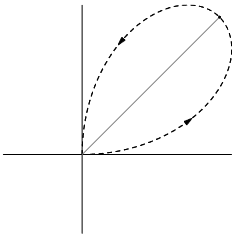
\includegraphics[scale=0.5]{03_un-petalo.jpg}
\end{figure}

Si ampliamos el intervalo a $0 \leq \theta \leq 2\pi$, podremos observar que la flor de cuatro pétalos se va formando de forma suavizada, partiendo por el primer cuadrante, después por el cuarto, luego por el tercero y finalmente por el segundo. Cada uno de ellos los transita a través del origen.

\newpage

\begin{figure}[hbt!]
\centering
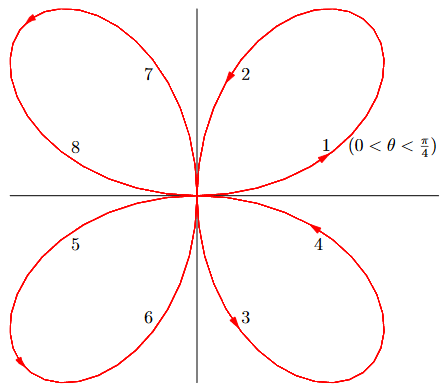
\includegraphics[scale=0.5]{04_rosa-cuatro-petalos.jpg}
\end{figure}

\end{document}
